%%%%%%%%%%%%%%%%%%%%%%%%%%%%%%%%%%%%%%%%%%%%
%
%	Institute of Financial Management
%	Department of Business Mathematics and Data Science
% 	Examplary Latex Document for Writing a Seminar Paper, 
%   Bachelor or Master Thesis
%
%%%%%%%%%%%%%%%%%%%%%%%%%%%%%%%%%%%%%%%%%%%%
%
% 	This is an exemplary document that shall explain the 
%   professional use of Latex in a scientific application. 
%   Latex has the following advantages:
%
% 	1.) Dealing with mathematical notation:
% 	    Layout and writing equations are generally easier using LaTeX 
%       compared to other editors.
%
% 	2.) Consistent handling of intra-document references and bibliography: 
%	    While the major WYSIWYG editors can perform similar tasks, handling
%   	and consistency of numbering, cross-references, and bibliographic items
%       is easier and more flexible in LaTeX.
%
%	3.) Separation of content and style:
%		In principle this means that you can write your document without
%       caring about how it is formatted, and at the end of the day wrap 
%       it in the style-file provided by a journal publisher or University to
%       conform to the required style. 
%        
%	4.) Tables and illustrations:
%       LaTeX allows to easily include high quality graphics (.eps) and many
%       software packages (e.g. STATA) can produce output tables in latex format
%       such that they can be included without further formatting necessary. 
%
%		We highly recommend the usage of LaTeX as it is some kind of scientific
%       standard. The earlier you get used to it, the easier it will be for you
%       to hand in professional looking assignments and thesis papers. The 
%       following packages and commands are only a limited selection of what is
%       possible, but it will get you started. You may want to adapt the header
%       to your needs. If you have an idea but do not know how to implement it in
%       LaTeX, don't hesitate and try to google it. You will see that nearly any
%       problem that you may face has been discussed before and there are many
%       solutions available online.
%
%%%%%%%%%%%%%%%%%%%%%%%%%%%%%%%%%%%%%%%%%%%%


%%%%%%%%%%%%%%%%%%%%%%%%%%%%%%%%%%%%%%%%%%%%
%
%	(1.) Set Up a Document 		
%
%%%%%%%%%%%%%%%%%%%%%%%%%%%%%%%%%%%%%%%%%%%%

% 	Base LaTeX offers five classes of document: book, report, article
%   and letter. For each class, LaTeX provides a class file. The user 
%   arranges to use it via a \documentclass command at the top of the 
%   document. Additionally the user can specify the paper format and 
%   may change the font size.

\documentclass[a4paper,12pt]{article}
\linespread{1.5} 
\renewcommand{\footnotesize}{\fontsize{10}{11}\selectfont}
% 	After the document is set up, a variety of packages is loaded to 
%   customize the environment.

\usepackage[top=2.5cm, left=5cm, bottom=2cm, right=2.5cm]{geometry}

\usepackage[longnamesfirst, round]{natbib}  
%   The bun­dle pro­vides a pack­age that im­ple­ments both au­thor-year and
%   num­bered ref­er­ences, as well as much de­tailed of sup­port for other
%   bib­li­og­raphy use.

\usepackage[latin1]{inputenc}   
% 	The pack­age trans­lates var­i­ous stan­dard and other in­put en­cod­ings
%   into a ‘LATEX in­ter­nal lan­guage’. The in­ter­nal lan­guage is ex­pressed
%   en­tirely in TEX's base en­cod­ing (stan­dard ASCII print­able char­ac­ters,
%   car­riage con­trol to­kens and TEX con­trol se­quences, the lat­ter 
%	mostly de­fined by LATEX).
%   If German special characters are needed and do not work, try utf8
%   instead of latin1. Settings depend on your operating system.

\usepackage[T1]{fontenc}        
%	The pack­age al­lows the user to se­lect font en­cod­ings, and for each
%   en­cod­ing pro­vides an in­ter­face to ‘font-en­cod­ing-spe­cific’ com­mands 
%   for each font. Its most pow­er­ful ef­fect is to  en­able hy­phen­ation 
%   to op­er­ate on texts con­tain­ing any char­ac­ter (especially umlaut) 
%   in the font.

\usepackage{color}              
%	The color pack­age pro­vides both fore­ground (text, rules, etc.) and 
%   back­ground colour man­age­ment; it uses the de­vice driver con­fig­u­ra­tion 
%   mech­a­nisms of the graph­ics pack­age to de­ter­mine how to con­trol its oup­tut.

\usepackage{amsmath,amsfonts,amssymb}   
%	The prin­ci­pal pack­age in the AMS-LATEX dis­tri­bu­tion. It adapts for 
%   use in LATEX most of the math­e­mat­i­cal fea­tures found in AMS-TEX; it 
%   is highly rec­om­mended as an ad­junct to se­ri­ous math­e­mat­i­cal type­set­ting 
%   in LATEX. When ams­math is loaded, AMS-LATEX pack­ages ams­bsy (for bold 
%   sym­bols), am­sopn (for op­er­a­tor names) and am­s­text (for text em­bed­ded in 
%   math­e­mat­ics) are also loaded.

%\usepackage{ngerman}           
%	Sup­ports the new Ger­man or­thog­ra­phy (neue deutsche Rechtschrei­bung).

\usepackage[english]{babel}     
% 	The pack­age pro­vides the lan­guage def­i­ni­tion file for sup­port of English
%   in ba­bel. Care is taken to se­lect british hy­phen­ation pat­terns for Bri­tish
%   English and Aus­tralian text, and de­fault (‘amer­i­can’) pat­terns for Cana­dian
%   and USA text.

\usepackage{ae}                 
%	A set of vir­tual fonts which em­u­lates T1 coded fonts us­ing the stan­dard CM
%   fonts. The pack­age name, AE fonts, sup­pos­edly stands for “Al­most Euro­pean”.
%   The main use of the pack­age was to pro­duce PDF files us­ing Adobe Type 1 
%   ver­sions of the CM fonts in­stead of bitmapped EC fonts.

\usepackage{graphicx}           
% 	The pack­age builds upon the graph­ics pack­age, pro­vid­ing a key-value 
%   in­ter­face for op­tional ar­gu­ments to the \in­clude­graph­ics com­mand. It allows
%   to include graphics in all conventional formats (pdf, jpg, tif, ...).

\usepackage{epstopdf}
%	Allows to include .eps graphics which are converted on the fly to pdf.

\usepackage{longtable}          
% 	Longtable al­lows you to write ta­bles that con­tinue to the next page. 
%   You can write cap­tions within the ta­ble (typ­i­cally at the start of the 
%   ta­ble), and head­ers and trail­ers for pages of ta­ble. Longtable ar­ranges
%   that the columns on suc­ces­sive pages have the same widths.

\usepackage{booktabs}
% 	Allows to set nice vertical lines in the table environment.

\usepackage[flushleft]{threeparttable}
%	Allows to nicely write a description at the bottom of a table

\usepackage{multirow}         
% 	Allows to connect rows in tables.

\usepackage{url}
%	The com­mand \url is a form of ver­ba­tim com­mand that al­lows line­breaks
%   at cer­tain char­ac­ters or com­bi­na­tions of char­ac­ters, ac­cepts 
%   re­con­fig­u­ra­tion, and can usu­ally be used in the ar­gu­ment to an­other 
%   com­mand. The com­mand is in­tended for email ad­dresses, hy­per­text links, 
%   di­rec­to­ries/paths, etc., which nor­mally have no spaces, so by de­fault 
%   the pack­age ig­nores spaces in its ar­gu­ment. How­ever, a pack­age op­tion 
%   “al­lows spaces”, which is use­ful for op­er­at­ing sys­tems where spaces 
%   are a com­mon part of file names.

\usepackage{setspace}
%   Provides commands to adjust line spacing.

\usepackage{pdfpages}
%   Allows to include the pdf of the examinations office
%   (Eigenstaendigkeitserklaerung)

\usepackage{enumitem}

\usepackage{amsmath}

\usepackage{xurl}
\usepackage[font=small,skip=5pt]{caption}
\usepackage{titlesec}
%%%%%%%%%%%%%%%%%%%%%%%%%%%%%%%%%%%%%%%%%%%%
%
%	(2.) Further Document Definitions 		
%
%%%%%%%%%%%%%%%%%%%%%%%%%%%%%%%%%%%%%%%%%%%%

\bibliographystyle{abbrvnat}    
%	Defines the style of the bibliography.

\oddsidemargin 0.1in \evensidemargin 0.1in \textwidth 15.5cm \topmargin -0.4in \textheight 24.5cm   
% 	Defines width of margins. 

\parindent 0cm  
% Defines indentation at the beginning fo a new paragraph.

\pagestyle{plain}          
% 		Empty header line, page number in the center of the footer line.

\newcommand{\bs}{\boldsymbol}  
% 		Shortcut to produce fat symbols in the math environment

\usepackage{blindtext}

%%%%%%%%%%%%%%%%%%%%%%%%%%%%%%%%%%%%%%%%%%%%
%
%	(3.) Beginning of Document		
%
%%%%%%%%%%%%%%%%%%%%%%%%%%%%%%%%%%%%%%%%%%%%
\numberwithin{equation}{section}
\begin{document}

\onehalfspacing
% Sets the line spacing to 1,5

%%%%%%%%%%%%%%%%%%%%%%%%%%%%%%%%%%%%%%%%%%%%
%
%	(4.) Title page		
%
%%%%%%%%%%%%%%%%%%%%%%%%%%%%%%%%%%%%%%%%%%%%

% In principle you can design the title page on your own. The following requirements should however
% be met: Centered title and description, information about the author and date listed on the title page.

\pagenumbering{roman}   
% 		Use roman numbers for page numbering 

\begin{titlepage}       
% 		Wrapper for title page definitions

\thispagestyle{empty}   
% 		No page numbering on the title page

% 		Title page text that shall be displayed in the center of the page
\begin{center}
   \vspace*{2.5cm}
   {\bf  \Large Challenges in Assessing Probabilistic Classifiers: \\ROC Curves and Beyond} \\
   \vspace*{3cm} 
   Term paper for the \\ Data Analytics Seminar\\ Winter Term 2023/2024\\
   Chair of Econometrics and Statistics\\ 
   University of Hohenheim
   % adapt to your needs and give the appropriate information 
   \end{center}


%		Information about the author of the thesis
\vfill

\hfill \begin{minipage}{0.5\linewidth}
 First examiner: M.Sc. Marius Puke \\
 Second examiner: Prof.\ Dr.\ Thomas Dimpfl \\
 % examiners only needed for master thesis
 
 Submitted by: Noemi Avello \\
 Student Number: 998749 \\
 
 Date of Submission: \today 
\end{minipage}


\end{titlepage}

\newpage                 
% Enforces a page break

%%%%%%%%%%%%%%%%%%%%%%%%%%%%%%%%%%%%%%%%%%%%
%
%	(5.) Table of Contents		
%
%%%%%%%%%%%%%%%%%%%%%%%%%%%%%%%%%%%%%%%%%%%%

%	Includes a table of contents and a list of your figures and tables.
\tableofcontents

%   In most journal publications, none of these is actually used.
\newpage

%%%%%%%%%%%%%%%%%%%%%%%%%%%%%%%%%%%%%%%%%%%%
%
%	(6.) Main Body
%
%%%%%%%%%%%%%%%%%%%%%%%%%%%%%%%%%%%%%%%%%%%%

\pagenumbering{arabic}      
% 		Set page numbering back to arabic numbers
\setcounter{page}{1}  
% 		Set counter back to 1  

% 	You can use different levels of sections to structure the body of your work. 

\section{Introduction}
\label{Chapter:intro}  
Evaluating the prediction power of real-valued markers or features for binary outcomes is crucial in every field. Having diagnostic tools for evaluating and comparing predictive capacity is a prerequisite for creating and refining probability projections.\bigskip

Receiver Operating Characteristic (ROC) curves are essential tools for assessing the prediction power of variables, markers, or features in different contexts. When evaluating the effectiveness of probabilistic classifiers derived from statistical learning methods like random forest, ROC curves are frequently utilized. However, for a variety of reasons, this approach's interpretability is restricted. The monotonicity constraint on the conditional event probability, which is the foundation of the methodology and must be invoked to justify the building of any raw ROC diagnostic or ROC curve, is what gives concavity its crucial role in the understanding and modeling of ROC curves. \bigskip

This seminar paper describes how to apply a technique that subjects the marker or feature in question to pool-adjacent violators to morph ROC curves into their concave hull. In addition, it was evaluated some alternative techniques. \bigskip

The structure of the document is as follows. Some theory foundations for evaluating probability forecasts are established in Section 2, formally expressing the relationship between the probability forecast and the Conditional Event Probability (CEP) with calibration. Furthermore, as depicted visually in reliability diagrams, a probability forecast or probabilistic classifier is deemed reliable or calibrated if the anticipated probabilities correspond with ex-post observed frequencies. The traditional method of creating reliability diagrams by binning and counting has been hindered by its inability to maintain stability in the face of unforeseen, unsystematic implementation decisions. As a result, the CORP approach which produces automatically generated, appropriately binned, reproducible, and statistically consistent reliability diagrams is included in this section. In Section 2, the differences between ROC curves and raw diagnostics are discussed, along with the particular importance of concavity in ROC curve modeling and interpretation. Two ROC alternatives, precision-recall curves, and MCB-DSC plots are covered in Section 3 to examine alternative evaluation techniques with different advantages despite the same objective.\bigskip

The seminar paper closes in Section 4, which discusses an empirical application using real-world data of vehicle loan default used in a Hackathon competition in 2019. Data on forecasts and seminar application have been deposited at GitHub (\url{https://github.com/TimoDimi/replicationDGJ20}).


\section{Basics in probability forecast evaluation}
\label{Chapter:Probability forecast}  
%   The label allows you to later reference this Section using \ref{Chapter:intro}. 
%   If at any stage you insert another section before, the reference is 
%   automatically updated.

Probabilistic forecasts provide a predicted probability distribution for a forthcoming item or event, taking into account forecast uncertainty. A future binary or dichotomous occurrence, such as a credit default or not credit default, or the likelihood of a precipitation occurrence in the future is the most straightforward scenario (\cite{Forecast2}). Predictive probability distribution in the binary situation is only the ex-ante likelihood, or the event to occur. \bigskip

Assigning a positive result as $Y = 1$ and a negative result as $Y = 0$. A probability forecasting for $Y$ may have a probability $p \in [0.1]$ for a positive outcome.

   \subsection{The CEP} \label{Chapter:CEP}  
   The Conditional Event Probability (CEP) function addresses the task of predicting an outcome not yet observed, denoted by the random variable $Y$, ranging between 0 and 1 based on a set of observables $X$. The likelihood of $Y$ being 1 given $X$ equal to $x$ is analogous to both the conditional mean and the distributional forecast for the binary outcome $Y$.
         
   \begin{equation} \label{eq:CEP} 
   CEP(x) = \mathbb{Q}(Y = 1 | X = x)
   \end{equation}
  
   In probability forecasting, the objective is to maximize the prediction distributions' sharpness, subject to calibration (\cite{Forecast1}).

   \subsection{Calibration}
   The degree to which conditional event frequencies agree with prediction probabilities is known as calibration or reliability, typically assessed via a graphical analysis.

      \subsubsection{Probability forecast and CEP relation for calibration}
      A forecast quality or performance can present different attributes with their respective measures. Calibration or reliability is a fundamental necessity for any probability forecast or probabilistic classifier. Essentially, a probabilistic classifier assigns a predictive probability to an occurrence of binary events. \bigskip

      Defining, the expected value of $Y$ given the forecast $X$:
      \begin{equation} \label{eq: expected} 
      \mathbb{E}[Y | X = x] 
      \end{equation}

      A probability forecast achieves calibration or is reliable when, under the condition of any forecast value $p$, the event materializes in 100 times $p$ percent of the instances under consideration. This means,
      
      \begin{equation} \label{eq: calibration} 
      CEP(x) = \mathbb{Q}(Y = 1 | X = x) = \mathbb{E}[Y | X = x]
      \end{equation}

      Thus, the probability forecast $X$ is calibrated if the function is equal to the forecast value $x$ for all relevant $x \in [0, 1]$. This criterion serves as a cohesive representation of calibration for binary outcomes. For instance, if we consider all cases with a predictive probability of about 0.60, the observed event frequency ought to be about 0.60 as well.

      \subsubsection{How to assess calibration}
      {\bf (i) Reliability diagrams\\}
      Conditional empirical event frequency versus forecast probability is plotted in one of the most well-known empirical calibration curve displays, demonstrating the possibility of an uncalibrated forecast when there are notable departures from the diagonal.\bigskip

      The "binning and counting" method, which begins by choosing a specific, usually arbitrary number of bins for the forecast values, is the foundation of the classical reliability diagram (\cite{reliability1}). Then, the corresponding conditional event frequency for each bin is plotted against the average prediction value or midpoint of the bin. \bigskip
      
      Despite being simple to use, the traditional method of generating reliability diagrams can be quite sensitive to the bin specifications, and even the smallest alteration can have a significant impact on the visual representation. As a result, instability is a significant problem that is usually brought on by several instances of the same prediction value at bin breaks. Additionally, the instabilities affect related numerical calibration metrics like the Brier-score reliability.\bigskip

      {\bf (ii) CORP reliability diagram\\}
      Based on nonparametric isotonic regression and the Pool-Adjacent-Violators (PAV) algorithm to estimate Conditional Event Probabilities (CEPs), the CORP approach produces provably statistically consistent, optimally binned, and reproducible reliability diagrams in an automated manner. This results in a fully automated choice of bins that adapts to both discrete and continuous settings, without any need for tuning parameters or user intervention.\bigskip

      In addition, the CORP diagram includes quantitative measurements of uncertainty (UNC), discrimination ability (DSC), and (mis)calibration (MCB), which outperform the traditional Brier-score decomposition in terms of stability (\cite{roc1}). A histogram showing the forecast values' unconditional distribution is typically added to the reliability curve.\bigskip

      The basic idea of CORP is to use nonparametric isotonic regression to estimate a forecast's CEPs as a monotonic, non-decreasing function of the original forecast values. To each original forecast value, the PAV algorithm assigns a (re)calibrated probability under the regularizing constraint of isotonicity, and this solution is optimal under a very broad class of loss functions. In particular, the PAV solution constitutes both the nonparametric isotonic least squares and the nonparametric isotonic maximum-likelihood estimate of the CEPs.\bigskip

      For a specific form record, \begin{equation} \label{e:record} \left( x_{1},y_{1}\right),...,\left(x_{n},y_{n} \right)\end{equation} Assume, without losing generality, $x_{1} \leq ... \leq x_{n}$, and let 
      
      \begin{equation} \label{e:recalibrated} 
      \hat{x_{1}} \leq ... \leq \hat{x_{n}}
      \end{equation}

      represent the values that the PAV algorithm recalibrated. The piecewise linear curve that connects the points $(x_{1},\hat{x_{1}}),...,(x_{n},\hat{x_{n}})$ is shown in the CORP reliability diagram. When the original forecast is calibrated, the reliability curve is on the diagonal, and  $x_{1} = \hat{x_{1}},...,x_{n} = \hat{x_{n}}$. In every other case, consistent departures from the diagonal point to a lack of calibration. Curves below the diagonal overestimate the predictions and above the diagonal  underestimate.\bigskip

      CORP reliability diagrams are provably statistically consistent, in contrast to the binning and counting method, which has not been the subject of asymptotic analysis. Moreover, CORP is asymptotically efficient, meaning that an estimate as accurate as feasible in the large sample limit is produced by its automatic binning decision.\bigskip

      {\bf (ii.1) CORP Score Decomposition\\}
      The CORP decomposition decomposes a mean score 
      
      \begin{equation} \label{e:sdecomposition} 
      \bar{S} = MCB -DSC + UNC 
      \end{equation}


      the miscalibration element MCB represents the variation in mean scores between the first and (re)calibrated forecasts showing the degree to which the conditional event frequencies and predicted probabilities diverge. In the same direction, the DSC component evaluates a prediction's capacity to discriminate between events and non-events by calculating the difference between the mean score for the reference and the (re)calibrated forecast. Large values of the DSC component are also desirable, in addition to small values of the MCB. The traditional measure of uncertainty (UNC), which is independent of the forecast being examined is just the reference forecast's mean score used to evaluate the intrinsic complexity of the prediction task.\bigskip

      As before, let $\hat{x_{1}} \leq ... \leq \hat{x_{n}}$ represent the PAV re-calibrated values from equation (\ref{e:recalibrated}), as depicted in the CORP reliability diagrams, and for a given record (\ref{e:record}), assume without loss of generality that $x_{1} \leq ... \leq x_{n}$. Additionally, let the realized unconditional event frequency be represented by $r = \bar{y} = \frac{1}{n} \sum_{i=1}^{n} y_{i}$. $S$ serving as any appropriate scoring guideline, let's 

      \begin{equation} \label{e:scoring}
      \bar{S}_{C} = \frac{1}{n} \sum_{i=1}^{n} S(\hat{x_{i}},y_{i}) \text{ and } \bar{S}_{R} = \frac{1}{n} \sum_{i=1}^{n} S(r,y_{i})
      \end{equation}

      indicate, respectively, the mean score for the constant Reference prediction $r$ and the (re)Calibrated probability. The average score $\bar{S} = \frac{1}{n} \sum_{i=1}^{n} S({x_{i}},y_{i})$ splits down as (\cite{roc1}) 

      \begin{equation} \label{e:dec_scoring}
      \bar{S} = \underbrace{(\bar{S} - \bar{S}_{C})}_{\text{MCB}} - \underbrace{(\bar{S}_{R} - \bar{S}_{C})}_{\text{DSC}} +  \underbrace{\bar{S}_{R}}_{\text{UNC}}
      \end{equation}

      The resulting decomposition of the mean score is exact and ensures that $DSC \geq 0$ with equality if the (re)calibrated forecast is constant, and $MCB \geq 0$  with equality if the initial forecast is calibrated.\bigskip

      Specifically, the CORP score decomposition, never produces paradoxical negative values of the components. Parts away from the diagonal suggest a lack of calibration, whereas extended horizontal segments are indicative of diminished discriminating ability. These situations of vanishing components ($MCB = 0$ or $DSC = 0$) confirm the intuitive interpretation of CORP reliability diagrams.\bigskip

   \subsection{Discrimination analysis via ROC curve}
   In binary problems, receiver operating characteristic (ROC) curves are widely used to assess variables, markers, or characteristics as possible predictors. In a nutshell, ROC curves show prospective prediction capability independent of calibration factors.\bigskip

   The relationship between the Hit Rate (HR) and False Alarm Rate (FAR) as the decision threshold changes is plotted graphically via the ROC. Specifically, take into consideration the joint distribution $\mathbb{Q}$ of the pair $(X, Y)$, where $Y$ is a binary event and $X$ is a real-valued covariate, marker, or feature. It is implicitly understood that larger values of $X$ give stronger support for the event to materialize $(Y = 1)$ the prevalence $\pi_{1} = \mathbb{Q}(Y=1)\ \in \ (0,1)$ and the conditional Cumulative Distribution Functions (CDFs) define the joint distribution $\mathbb{Q}$ of $(X, Y)$.

   \begin{equation} \label{e:distribution} 
   F_{1}(x) = \mathbb{Q}(X\leq x)|Y=1) \text{ and } F_{0}(x) = \mathbb{Q}(X\leq x)|Y=0)
   \end{equation}

   A classifier with a Hit Rate (HR), can be produced by using any threshold value $x$ to predict a positive result $(Y = 1)$ if $X > x$ and a negative outcome $(Y = 0)$ if $X \leqslant   x$.

   \begin{equation} \label{e:hit_rate} 
   HR(x) = \mathbb{Q}(X>x | Y=1) =1 - F_{1}(x),
   \end{equation}

   and False Alarm Rate (FAR),

   \begin{equation} \label{e:far} 
   FAR(x) = \mathbb{Q}(X>x | Y=0) =1 - F_{0}(x)
   \end{equation}

   FAR is the probability of making a false positive decision, whereas HR is that of making a correct positive decision.\bigskip

   ROC curves consider all potential thresholds, making them helpful for comparing different classifiers. It is desirable to have high hit rates and low false alarm rates, hence it is best if the ROC curve approaches the upper left corner of the unit square. A common metric for assessing a feature's potential predictive usefulness is the Area Under the ROC Curve (AUC).

   \subsubsection{The Area Under the Curve (AUC)}
   The area under the ROC curve measure is a widely used method in scientific publications to compare the prediction abilities of probabilistic classifiers (\cite{roc3}). The likelihood that a value randomly selected from the empirical distribution of prediction values for an event will be greater than a value selected from the distribution for a non-event is an attractive interpretation of AUC.\bigskip
   
   Perfect discriminating ability is indicated by an AUC value of 1; no discrimination is indicated by a $\frac{1}{2}$ matching to the diagonal trivial ROC curve. If the value is less than $\frac{1}{2}$, it suggests that the accuracy of the forecast could be increased by changing the forecasts for $0$ and $1$. AUC is invariant under strictly increasing transformations, just as the ROC curve is, and it is noted that AUC exclusively concerns discrimination ability, while ignoring (mis)calibration (\cite{roc1}).

   \begin{figure}[hbt!]
      \centering
      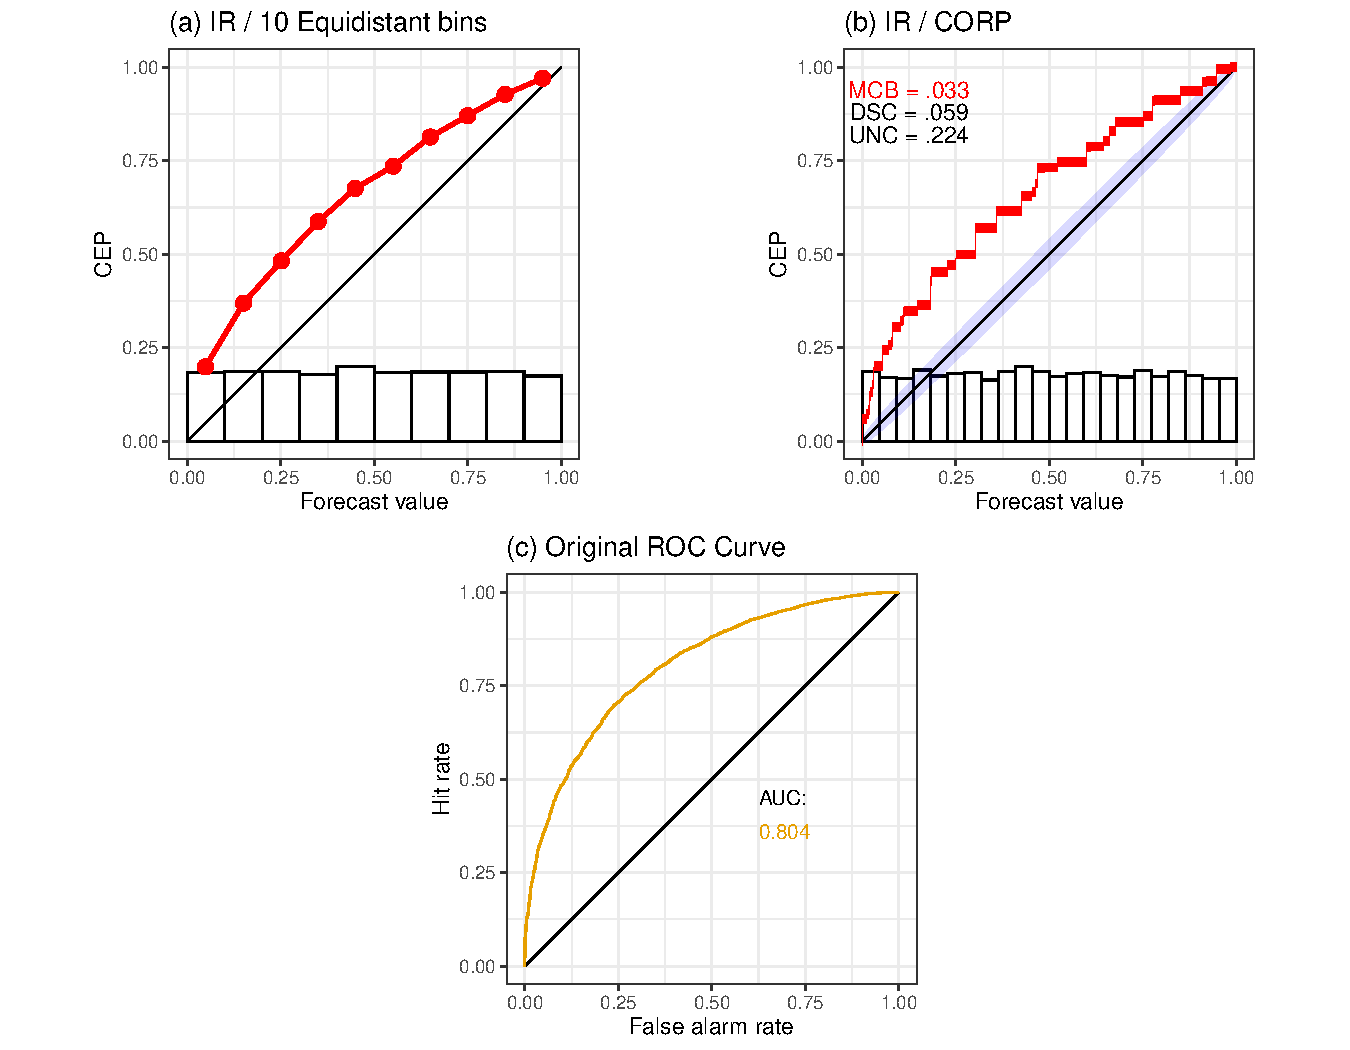
\includegraphics[scale=0.65]{Plots_sim/layout1.pdf}
      \caption{Reliability diagrams (a and b). Under the binning and counting approach, a reliability diagram is displayed with 10 equally spaced bins for selection (a). Furthermore, a CORP reliability diagram (b). The forecast values for n = 92 are displayed as a distribution in the histograms at the bottom. The original ROC curves for the forecasts $x_{1},...,x_{n}$ from (\ref{e:record}) are displayed in Panel (c).}
      \label{fig:layout1}
  \end{figure}


   \subsubsection{Raw ROC diagnostics and ROC curves}
   In order to understand the unique function of concavity in reading and modeling ROC curves, we must distinguish between raw ROC diagnostics and ROC curves.\bigskip

   ROC diagnostics in this typical context address the form's points $(FAR(x), HR(x))^{'},$ where $FAR(x)=1-F_{0}(x)$ is the false alarm rate and $HR(x)=1-F_{1}(x)$ the hit rate at the level of the threshold $x \ \in \ \mathbb{R} $. Formally, the point set is the raw ROC diagnostic for the bivariate distribution $\mathbb{Q}$ and the random vector $(X, Y)$ (\cite{roc2}).

   \begin{equation} \label{e:bivariate} 
   R^{*} = \left\{ \binom{1-F_{0}(x)}{1-F_{1}(x)}: x \  \epsilon \  \mathbb{R} \right\}  
   \end{equation}

   inside the square of units. $F_{0}$, $F_{1}$, and either of the two marginal distributions clearly characterize the bivariate distribution $\mathbb{Q}$ of $(X, Y)$. However, because of the well-known invariance of ROC diagnostics under strictly increasing transformations of $X$ and variations in the predominance of the binary outcome, the raw ROC diagnostic combined with a single marginal does not represent $\mathbb{Q}$. Nonetheless, $\mathbb{Q}$ is determined by combining the two marginal distributions and the raw ROC diagnosis.\bigskip
   \newpage
   Linear interpolation is used to create a ROC curve from the raw ROC diagnostic. Specifically, the utilization of linear interpolation enables an equitable and straightforward comparison of continuous, discrete, and ordinal data.\bigskip

   For the illustration of reliability diagrams and raw ROC diagnosis, a data set was simulated, where $x$ has a uniform distribution $x \thicksim  U(0,1)$, the calibration curve of $p(x)$ is $p(x)^{0,5}$, $y$ is binomial with $(n, 1, p(x))$, and choosing an $n$ equal to 10000. Figure \ref{fig:layout1} illustrates reliability diagrams based on the binning and counting approach with a choice of m = 10, the CORP reliability diagrams also displaying measures of (most importantly, and hence highlighted) (mis)calibration (MCB), discrimination (DSC), and uncertainty (UNC), and the raw ROC curve using isotonic regression (IR). \bigskip

   In real-world settings, this nearly perfect situation shown in the simulation will not hold, as illustrated \cite{roc2}, \cite{roc3}, and \cite{roc1}, reports ROC curves that are not always increasing. In addition, Fig 4.8 in \cite{statistical} on page 151 provides ROC curves that fail to be concave. The concavity of ROC curves is a factor that is frequently ignored yet is crucial. However, there can be a different approach technique to obtain concave hull ROC curves to get sensible plots to have better decision-making.

   \subsubsection{Concave ROC curves }
   The concavity of ROC curves is a valuable but frequently overlooked factor. It is nearly always the case that the original ROC curves created using empirical data are not concave. When the conditional event probability is nondecreasing with the forecast value $x$, which is rarely the case for empirical data, a ROC curve is concave. ROC curves measure prospective predictive ability or discrimination capacity. Although potential predictive ability does not depend on calibration, it can only be evaluated in the case of bigger prediction values, which are indicative of higher occurrence probabilities. \bigskip

   The ROC curve's concavity suggests right away that the area under the curve is a closed convex set, which includes the curve itself. The area under the curve can be readily demonstrated to be strictly convex if the ROC curve is strictly concave. Any convex combination of points in the area under and on the curve in this situation will be under the curve.\bigskip

   Assuming that $F_{1}$ and $F_{0}$ have continuous, strictly positive Lebesgue densities $f_{1}$ and $f_{0}$ in the interior of an interval, which is their common support, we obtain the regular setup (\cite{roc2}).\bigskip
   \newpage
   The likelihood ratio can be defined for each $x$ in the interior of the support,

   \begin{equation} \label{e:likelihood} 
   LR(x) = \frac{f_{1}(x)}{f_{0}(x)} 
   \end{equation} 

   and the conditional event probability,

   \begin{equation} \label{e:conditional} 
   CEP(x) = \mathbb{Q}(Y=1 | X=x) = \frac{\pi_{1}f_{1}(x)}{\pi_{0}f_{0}(x) + \pi_{1}f_{1}(x)}
   \end{equation}

   It can be shown that in  the regular and discrete settings statements (a), (b), and (c) are equivalent (\cite{roc2}):

   \begin{enumerate}[label=(\alph*)]

   \item The ROC curve is concave.
   \item The likelihood ratio is nondecreasing.
   \item The conditional event probability is nondecreasing.
   \end{enumerate}
   
   A function $R: [0, 1] \rightarrow  [0, 1]$ can be used to identify the ROC curve in the standard setup, where $R(p)$ is defined as $R(p) = 1 - F_{1}(F_{0}^{-1}(1-p))$ for $p \in (0, 1)$. The function $R$ is evidently concave if the ROC curve is concave, and as a result, its derivative $R^{'}(p)$ is nonincreasing in $p \in (0, 1)$. The equivalency of (a) and (b), however, is established by the slope $R^{'}(p)$, which equals the likelihood ratio $LR(x)$ for a specific value $x$ that declines with $p$. Additionally,

   \begin{equation} \label{e:likelihood_ratio} 
   LR(x) = \frac{\pi_{0}}{\pi_{1}} \frac{CEP(x)}{1-CEP(x)}
   \end{equation}

   and in $c \in (0, 1)$, the function $c \rightarrow {c}/{1-c} $ is nondecreasing, producing the equivalency of (b) and (c).\bigskip

   The discrete situation, where the support of feature $X$ is either a countably infinite or finite set, is the next setting we look at. The case of empirical ROC curves is one example of this scenario, but it's not the only one. We can determine the likelihood ratio for each $x$ in the discrete support of $X$.
   
   \begin{equation} \label{e:sqasduared} 
      % \[
         LR(x) = \left\{\begin{array}{@{}lr@{}}
            \mathbb{Q}(X = x|Y=1)/\mathbb{Q}(X = x|Y=0) & \text{ if } \ \mathbb{Q}(X = x|Y=0)>0\\
            \infty, & \text{ if } \ \mathbb{Q}(X = x|Y=0)=0
             \end{array}\right\}
      %  \]
      \end{equation}
      
   
   and the conditional event probability,

   \begin{equation} \label{e:con_prob} 
   CEP(x) = \mathbb{Q}(Y = 1 | X = x)
   \end{equation}

   Concavity plays a crucial role in the interpretation and modeling of ROC curves because of the monotonicity condition (c) on the conditional event probability. This condition is fundamental to the methodology and must be used to support the creation of any raw ROC diagnostic or ROC curve.\bigskip
   
   However, the solution is quite straightforward. Instead of using the original forecasts, the pool-adjacent violators (PAV) can be used to compute the ROC curve, which then transforms into its concave hull the smallest concave curve which is located to its upper left. Thus, the PAV algorithm converts into an isotonic, calibrated probabilistic classifier. Specifically, the PAV solution consists of the nonparametric isotonic maximum-likelihood estimate of the CEPs as well as the nonparametric isotonic least squares.

   \begin{figure}[h]
      \centering
      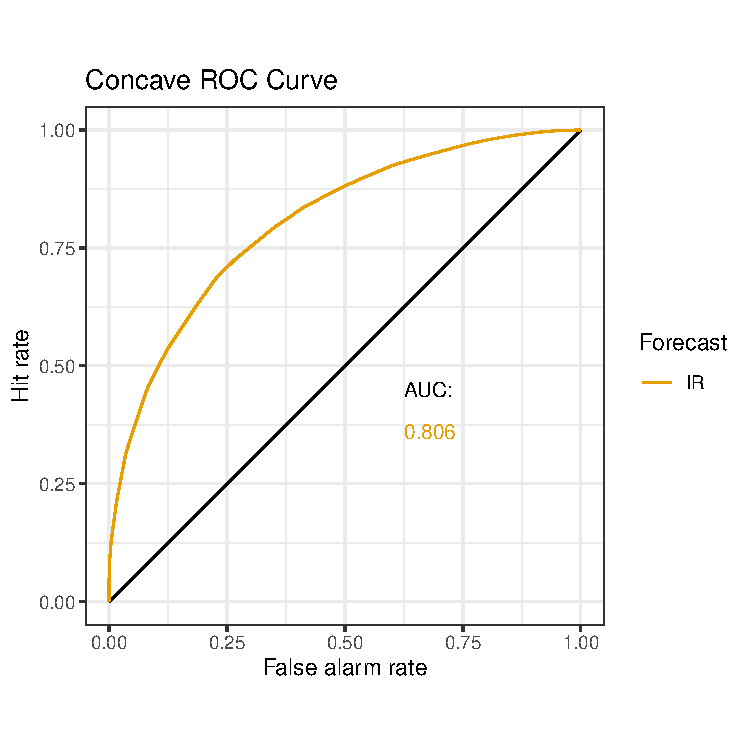
\includegraphics[scale=0.7]{Plots_sim/concave_sim.pdf}
      \caption{The original ROC curve transforms into its concave hull, as seen by concave ROC curves from the PAV re-calibrated forecasts.}
      \label{fig:concave_sim}
  \end{figure}

   Recalibrating removes variations in calibration, so the corrected, concave ROC curve is the only one used to measure discriminating ability, as illustrated in Figure \ref{fig:concave_sim}. On the other hand, conditional event frequencies that are not monotone have confusing effects, whereas the original ROC curves concentrate on discrimination abilities. A change in the ROC curve does not contradict the previously stated invariance under strictly increasing transformations because, in general, the transformation from the original probabilities $x_{1} \leq ... \leq x_{n}$ to the PAV transformed, recalibrated probabilities $\hat{x_{1}} \leq ... \leq \hat{x_{n}}$ is monotonic, but not strictly monotonic. \bigskip

   In conclusion, it is highly advised to employ concave ROC curves for empirical data, which are obtained from PAV-transformed forecast values. 

\section{ROC alternatives}

   \subsection{Precision-recall curves}
   For situations where there is a significant skew in the class distribution, like credit card fraud, the Precision-Recall (PR) curve might be used instead of ROC curves (\cite{precision}). A common scalar performance metric for contrasting various classifiers is the area under prediction-recall curves, which provide valuable insights into the effectiveness of binary classifiers.\bigskip 
   
   Therefore, to assess the performance of classifiers for imbalanced data sets, it is requires estimate recall and precision, 

   \begin{equation} \label{e:recall} 
   Recall = \frac{TP}{TP + FN} 
   \end{equation} 
   
   \begin{equation} \label{e:prec} 
   Precision = \frac{TP}{TP + FP}  
   \end{equation} \smallskip 

   where TP is true positives, FN false negatives, and FP false positives.

   \begin{figure}[h]
      \centering
      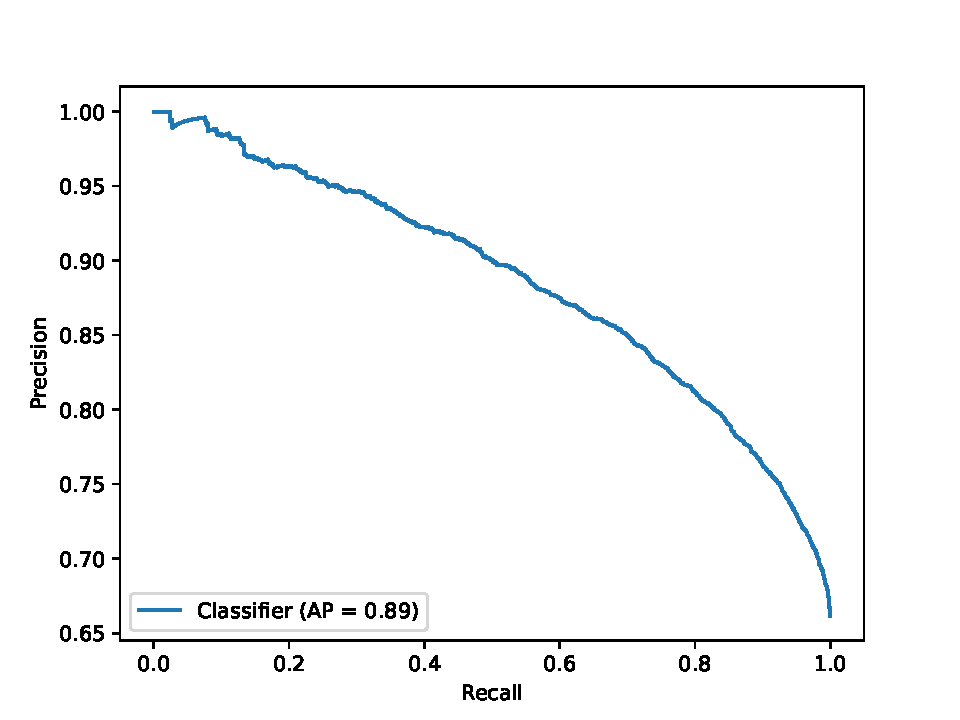
\includegraphics[scale=0.6]{Plots_sim/Precision_recall_sim.pdf}
      \caption{Precision-recall curve for simulated application.}
      \label{fig:Precision_recall_sim}
  \end{figure}

   Class imbalance has a direct impact on precision since it affects false positives, but the hit rate is only dependent on positives. For this reason, these impacts are not captured by ROC curves. PR curves therefore have a bigger benefit over ROC curves in skewed data instances where both precision and recall are critical.\bigskip 
   
   The area under the curve (AUC) measure, which is typically used to determine which classifier is superior, summarizes the performance of the classifier into a single quantitative measure. AUCs of superior classifiers are typically higher than those of weaker ones. Clear visual comparisons between two or more classifiers over a wide range of operational points are made possible by ROC and PR curves.

   \subsection{MCB-DSC plots}
   Plots of the calibration metric MCB against the DSC measure of discrimination ability show the performance of the classifier against several rivals. MCB-DSC plots help identify methods of interest by visualizing the strengths and limitations of forecasting methods through their simplicity and joint assessment of overall predictive ability, calibration, and discrimination. Therefore, the approach is recommended when a large amount of forecast methods need to be compared. The MCB-DSC plot utilizing brier and logarithmic score is displayed in Figure \ref{fig:mcb}, despite a single forecast.

   \begin{figure}[hbt!]
      \centering
      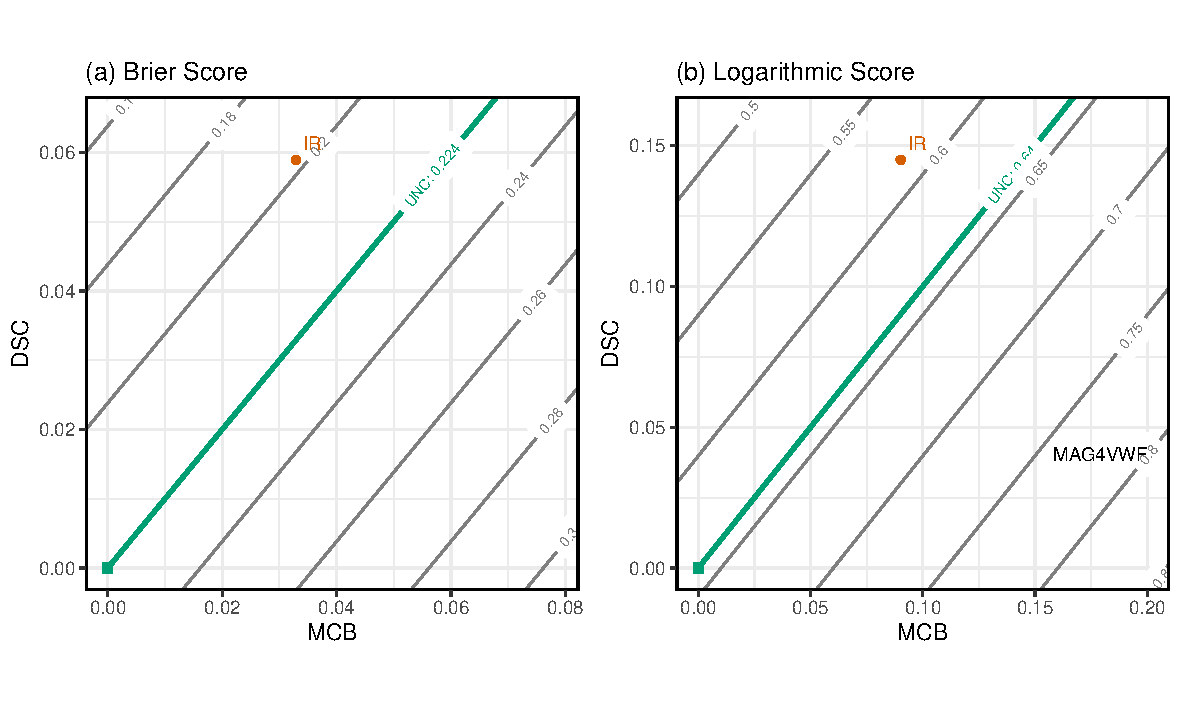
\includegraphics[scale=0.7]{Plots_sim/mcb.pdf}
      \caption{The Brier score and the logarithmic score are the two MCB-DSC graphs used to predict the likelihood of simulated data using isotonic regression. Forecasts that are better (above the line) and worse (below the line) than this baseline are distinguished by the thick green line. The green square at the origin represents the ex post best constant forecast, or the unconditional event frequency.}
      \label{fig:mcb}
  \end{figure}
   
   The difference between the mean score of the original and the (re)calibrated forecast is the miscalibration term $MCB = \bar{S} - \bar{S}_{C}$. It expresses variations in the score under evaluation from the diagonal of the CORP reliability curve. The discriminating component $DSC = \bar{S}_{R} - \bar{S}_{C}$ measures the extent to which the (re)calibrated prediction outperforms the reference score $\bar{S}_{R}$, which is derived from a calibrated but constant forecast (\cite{roc1}). It is noteworthy that DSC remains invariant under strictly increasing transformations of the forecast values under construction.
   
\section{Empirical application}
A real-world dataset of loan default predictions collected in India is used to support and empirically illustrate the theoretical explanation of  ROC curve challenges and beyond.\footnote[1]{Data source: https://www.kaggle.com/datasets/avikpaul4u/vehicle-loan-default-prediction}


   \subsection{Description of the data set}
   The vehicle loan default dataset provides information to predict the probability of borrowers defaulting on a vehicle loan on the due date of their first EMI (equated monthly installment). Furthermore, this dataset comprises three categories of borrower data: bureau data and history; loan information, including loan-to-value ratio, amount, and disbursal details; and borrower personal data, including age and type of job. This dataset contains 41 unique features in total. In terms of payback scenarios, $y = 0$ denotes no loan default and $y = 1$ denotes a loan default.\bigskip 

   The training set and test set are the two components of the loan default dataset. The test set is devoid of labels and just contains features because it was submitted as part of a Hackathon competition in 2019. 233154 observations make up the training set, which is the only one useful to be used. Of these findings, loan default occurs in 50611 cases (21.71\%).

   \subsection{Application}
   The data set explained in the previous section was manipulated to have data in the right format, consistent, and ready for model building. The main techniques applied to the vehicle loan default dataset were missing values and outliers treatment by applying a binning technique. In addition, feature selection drops useless features such as ID variables, data standardization, and dummy insertion to include categorical variables.\bigskip 
   
   To illustrate the seminar application through a real data set three models were applied, logistic model, Naive bayes (NB), and Random Forest (RF).

   \begin{figure}[hbt!]
      \centering
      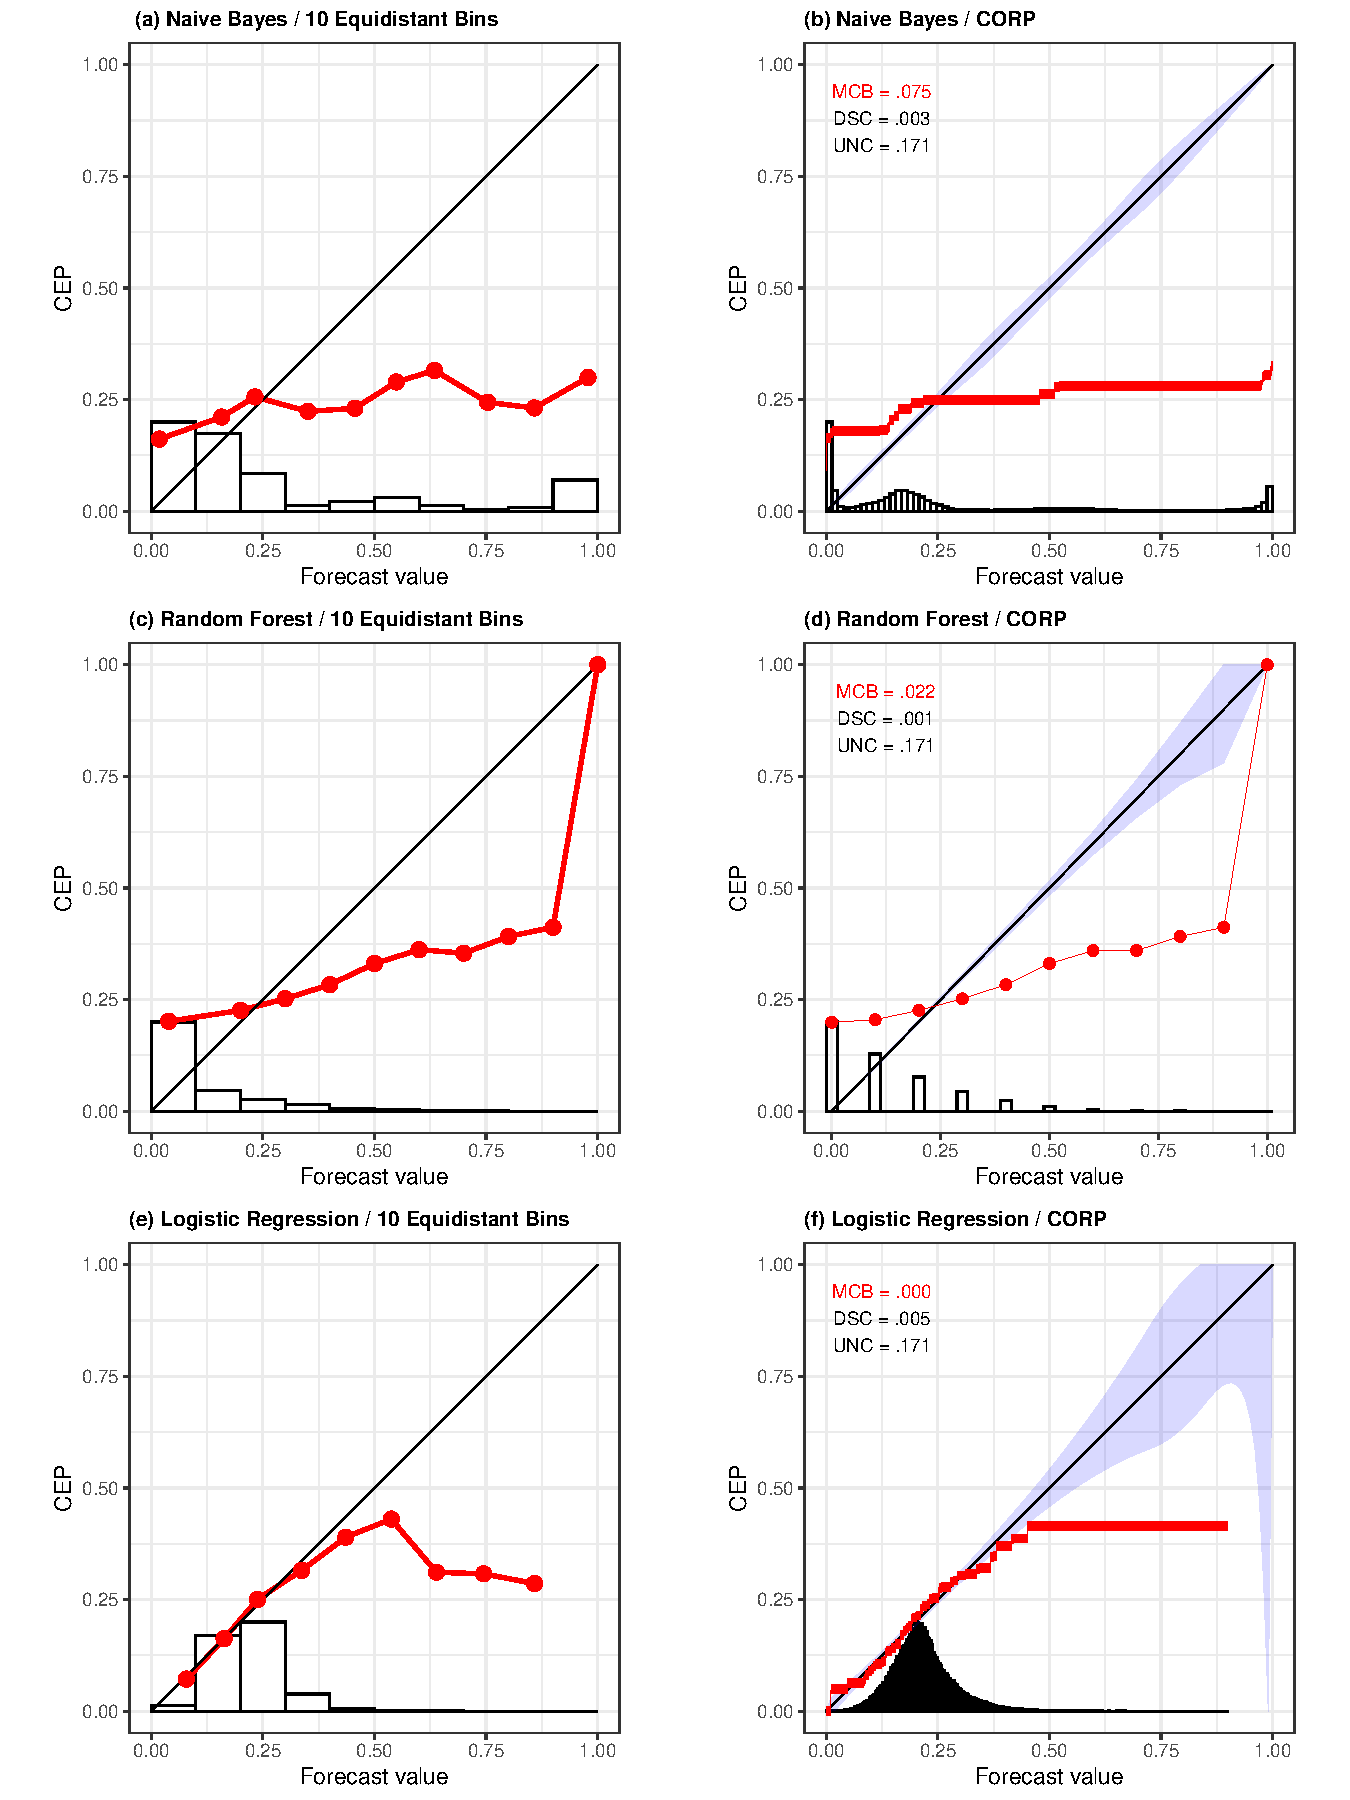
\includegraphics[scale=0.7]{Plots_app/layout3.pdf}
      \caption{Reliability diagrams based on the binning and counting approach were displayed in plots (a), (c), and (e). For each of the three models use m = 10 equally spaced bins. In addition, the CORP reliability diagrams in (b), (d), and (f) illustrate how the PAV-calibrated probability is plotted against the original prediction value.}
      \label{fig:rel_corp}
  \end{figure}

  \newpage
   The reliability diagram, which compares the predicted probability to the observed event frequency, is the primary diagnostic tool for assessing calibration mostly used in environments with limited prediction probabilities, such as discrete environments. However, the CORP reliability diagram which uses nonparametric isotonic regression and the Pool-Adjacent-Violators (PAV) algorithm to estimate Conditional Event Probabilities (CEPs), yields a fully automated choice of bins that adapts to both discrete and continuous settings, without any need for tuning parameters or implementation decisions, see Figure \ref{fig:rel_corp}. Furthermore, the plot provides the main variables in the CORP Brier-score decomposition for each model, being the logistic forecast the model with the best (smallest) MCB term and the best (highest) DSC component.\bigskip 

  The only ROC curve utilized to assess discriminating ability is the corrected, concave one since recalibrating eliminates calibration discrepancies. Conversely, non-monotonic conditional event frequencies have a confounding effect, while the original ROC curves focus on discriminatory power. Figure \ref{fig:roc_app} shows the concave ROC curve on the right side of the panel and the original version of the ROC curve on the left side for logistic, naive bayes, and random forest predictions.\bigskip 
  
  Since the transformation from the original probability to the PAV transformed, re-calibrated probabilities are often monotonic but not strictly monotonic, a change in the ROC curve does not contradict the previously established invariance under strictly rising transformations. Concave ROC curves, which are produced from forecast values that have been PAV-transformed, are highly recommended in conclusion.

  \begin{figure}[ht]
   \centering
   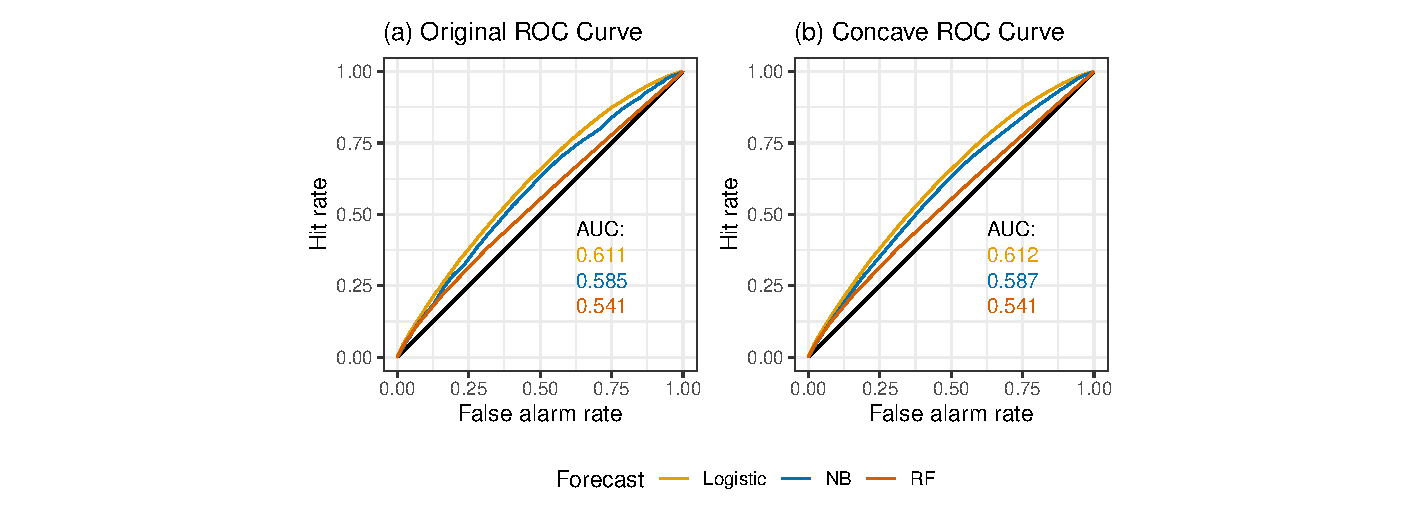
\includegraphics[scale=0.7]{Plots_app/ROC.pdf}
   \caption{Concave ROC curves from the PAV re-calibrated forecasts demonstrate that the original ROC curve morphs into its concave hull}
   \label{fig:roc_app}
  \end{figure}

 The Area Under the Precision-Recall Curve (AUC-PR) is the primary metric for assessing model performance due to the imbalanced nature of the dataset. The model with the highest AUC-PR was considered the best performer because higher PR-AUC values indicate better performance in identifying positive instances of loan defaulters. For the application, the logistic model is the best performer, as is shown in Figure \ref{fig:Precision_recall_app}. 
  
 \begin{figure}[h]
   \centering
   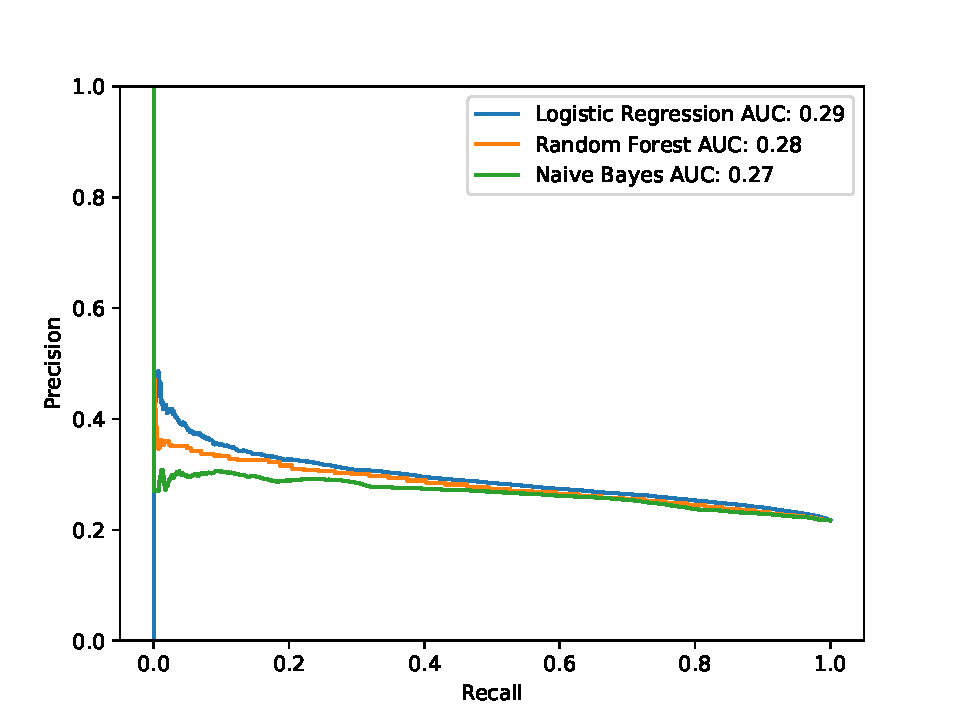
\includegraphics[scale=0.6]{Plots_app/Precision_recall_app.pdf}
   \caption{Precision-recall curves for logistic, random forest, and naive bayes models.}
   \label{fig:Precision_recall_app}
\end{figure}
  
The MCB-DSC plots, which display the DSC measure plotted against the MCB component for each competitor involved and are supplemented by parallel contour lines that denote an identical mean score, are useful for comparing a variety of competing forecasting techniques. Because of their ease of use and the way they jointly evaluate overall predictive ability, calibration, and discrimination, MCB-DSC plots help to visualize the advantages and disadvantages of forecasting techniques. 

   \begin{figure}[hbt!]
      \centering
      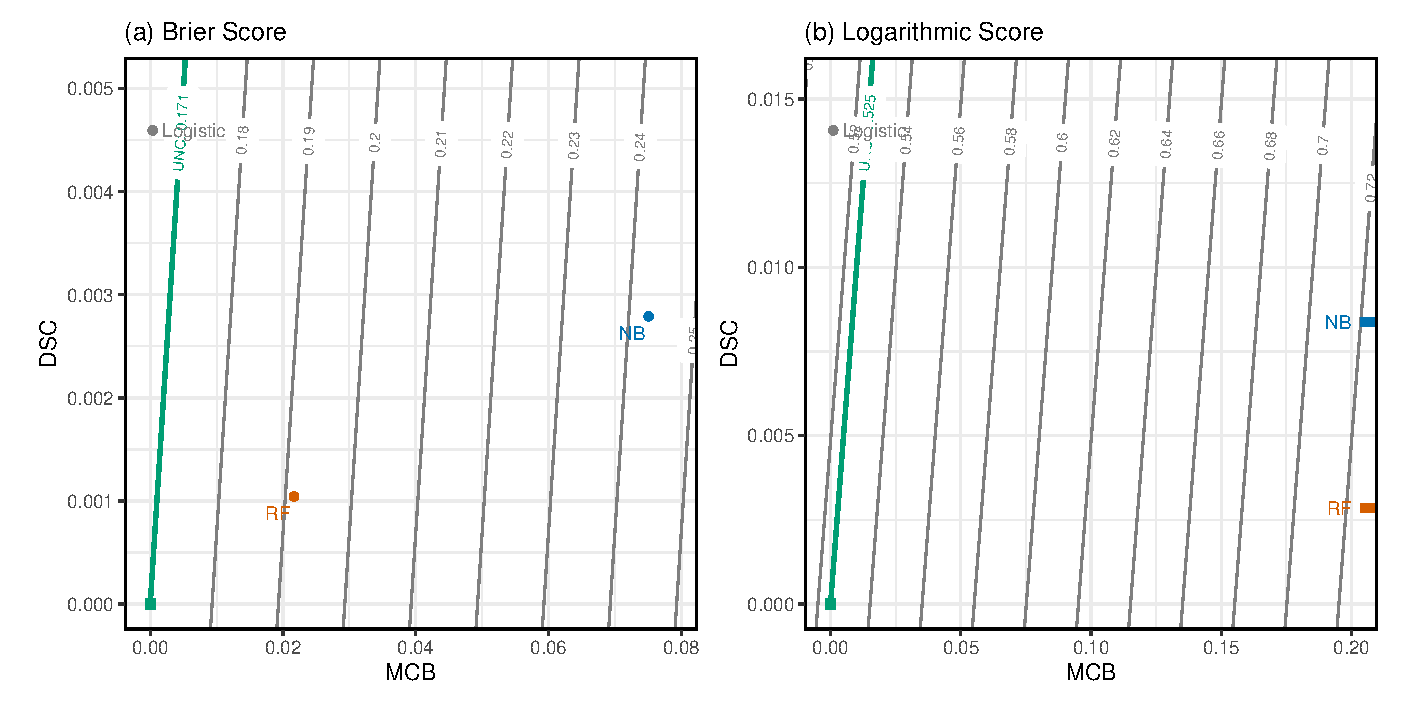
\includegraphics[scale=0.5]{Plots_app/app_MCBDSC.pdf}
      \caption{MCB-DSC plots for the logistic, naive bayes and random forest probability forecasts under (a) the Brier score and (b) the logarithmic score.}
      \label{fig:app_MCBDSC}
     \end{figure}

Brier score MCB-DSC plots for probability forecasts from logistic, random forest, and naive bayes forecasts are displayed in \ref{fig:app_MCBDSC}. It can be used the thick green line to separate forecasts that are better (above the line) and that are worse (below the line). For instance, only the logistic model is above the line, which is consistent with the previous analysis and the measures of MCB and DSC components. High DSC value but a low MCB metric. 


   \section{Conclusion}
   ROC curves have been widely used in many scientific fields to evaluate the potential predictive value of variables, features, or markers in binary scenarios. One of the desirable and appealing characteristics of ROC curves in this context is their ease of interpretation in terms of feasible operational circumstances; however, ROC curves are related to a concavity problem, and concavity is crucial to the interpretation and modeling of ROC curves.\bigskip 

   Nevertheless, the empirical ROC curve is produced by the PAV method from the corresponding concave hull. PAV-calibrated probabilities, given to the regularizing constraint of isotonicity, are optimal concerning any correct scoring technique. Furthermore, ROC curves offer several alternatives, such as MCB-DSC plots and Precision recall curves, which are mostly utilized for data sets that are unbalanced.\bigskip 
   
   The ROC curve concavity problem can be seen in the empirical application to highlight the limitations of ROC curves, and how concave fits are desirable, if not necessary, as they have nondecreasing conditional event probabilities and likelihood ratios for the predictor variables.\bigskip 
   
   The fitted logistic, naive bayes, and random forest ROC curves fail to be concave initially, but those change markedly towards morphing into its concave hull, when concavity is enforced using re-calibrated probabilities generated by the PAV algorithm.\bigskip 

   Examining the alternative evaluation techniques MCB-DSC plots, and precision-recall curves over the dataset, the results were consistent in the evaluation of discrimination ability between the models. MCB-DSC plots generate advantages when comparing multiple forecasts, however, in this context, its value is not as advantageous since it is only three models. In addition, precision-recall curves are mostly utilized for unbalanced data sets which is the case in this empirical application. \bigskip 
   
   However, it needs to be considered that the vehicle loan default dataset's imbalanced data set condition has an impact on this outcome. This gives room for improvement for further iterations.





%%%%%%%%%%%%%%%%%%%%%%%%%%%%%%%%%%%%%%%%%%%%
%
%										(7.) Required programs
%
%%%%%%%%%%%%%%%%%%%%%%%%%%%%%%%%%%%%%%%%%%%%

%%%%%%%%%%%%%%%%%%%%%%%%%%%%%%%%%%%%%%%%%%%%
%
%	(8.) Presentations
%
%%%%%%%%%%%%%%%%%%%%%%%%%%%%%%%%%%%%%%%%%%%%

%%%%%%%%%%%%%%%%%%%%%%%%%%%%%%%%%%%%%%%%%%%%
%
%	(9.) End of main body
%
%%%%%%%%%%%%%%%%%%%%%%%%%%%%%%%%%%%%%%%%%%%%


\newpage

%%%%%%%%%%%%%%%%%%%%%%%%%%%%%%%%%%%%%%%%%%%%
%
%	(10.) Bibliography
%
%%%%%%%%%%%%%%%%%%%%%%%%%%%%%%%%%%%%%%%%%%%%

\section{References}
%\addtocounter{section}{6}
%\addcontentsline{loc}{section}{References}

\bibliography{bibexample}                         % Creates a bibliography at the end of the LaTeX document. The bib-file loaded here is what you would have created with jabref. You can also give an absolute path if the bib-file is not in the folder where your tex-file lies. Same holds true for anything that is loaded by the way (figures, for example)

\newpage

%%%%%%%%%%%%%%%%%%%%%%%%%%%%%%%%%%%%%%%%%%%%
%
%	(11.) Appendix
%
%%%%%%%%%%%%%%%%%%%%%%%%%%%%%%%%%%%%%%%%%%%%

% You can include any of the two, irrespective of the language the 
% thesis is written.


\includepdf[scale=0.85,pages=1,pagecommand=\section{Appendix}]{declaration.pdf}

\includepdf[pages=2-,pagecommand={}]{declaration.pdf}

\end{document}
